\section{相关工作}
\label{section:relatedWork}
\subsection{eBPF}
扩展的伯克利包过滤器(extended Berkeley Packet Filter,eBPF)是一项基于事件驱动的Linux内核拓展技术,
支持动态地将用户编写的代码通过eBPF虚拟机加载到内核态上执行,而无需修改内核代码或者插入内核模块
\cite{sunFindingCorrectnessBugs2024, YIHeCrossContainer}。
这一直接运行于内核态而无需通过切换用户态和内核态之间的能力,既减少了数据复制次数提高了内核执行性能,又充分扩展了内核的功能
\cite{YIHeCrossContainer, ZhangZiJunLinuxXiTonge};
eBPF的这种灵活性被用于多种特定的任务\cite{HaoValidating},如网络包过滤\cite{10.1145/3371038, TCPdump}、
网络流量监控\cite{9110434}以及其它方面\cite{280870, 258973}。

\subsubsection{eBPF运行流程}
一个eBPF程序的运行流程如图 \ref{fig1} 所示。
用户首先需要编写包含BPF指令的程序段,通过BPF的系统调用加载BPF程序。
程序运行时只能操控11个寄存器(为R0至R10),只能在一个固定大小的栈上支持四种基本运算(加载、存储、算术运算和分支判断)
\cite{HaoValidating}。\nolinebreak
BPF程序经过加载时会经过编译工具链(如clang)编译为BPF字节码,而后经由BPF系统调用加载到内核态等待通过eBPF验证器的静态验证
\cite{zhengBpftimeUserspaceEBPF2023}。\nolinebreak
通过验证后,会经由BPF Just-In-Time(JIT)编译器编译为可执行的机器码并将其加载到虚拟机中执行。

\begin{center}
\begin{figure*}[t] 
    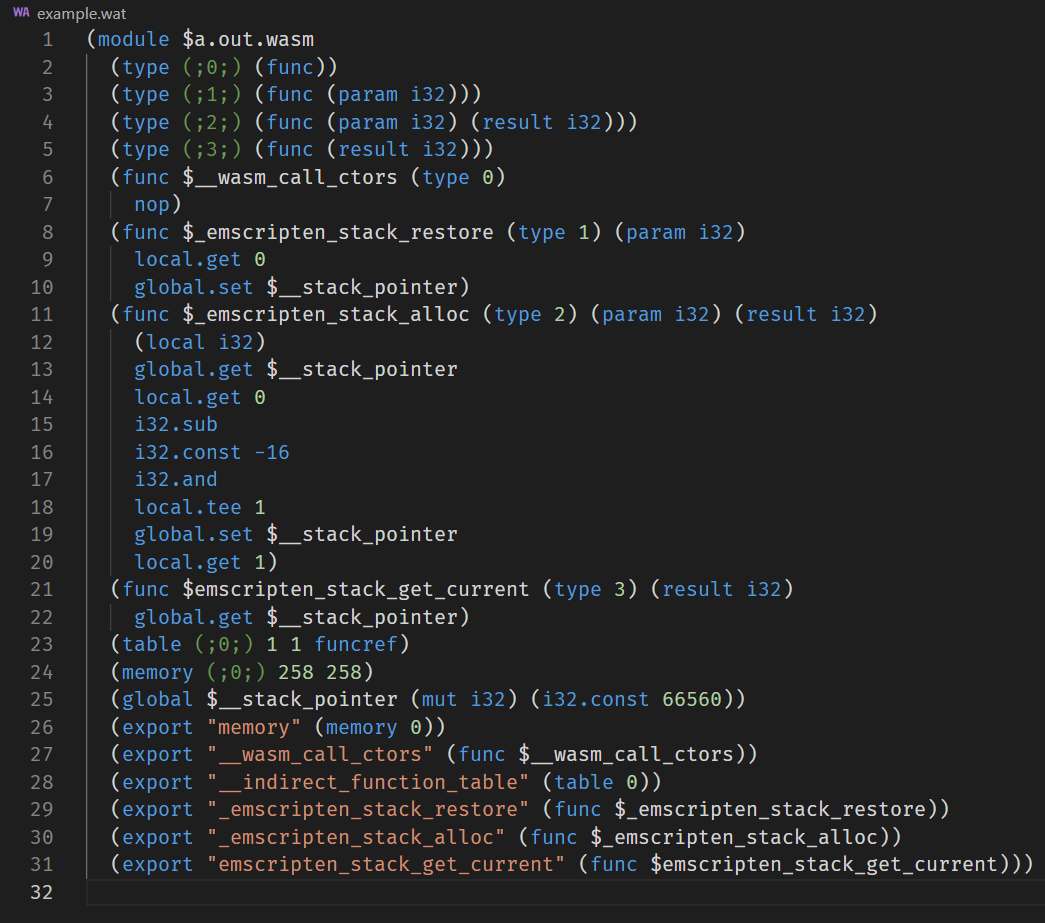
\includegraphics[width=0.1\textwidth]{fig1Codes.png}
    \caption{wasm对应的人类可读表示wat示意图}
    \label{fig1}
\end{figure*}
\end{center}

\subsubsection{eBPF存在的问题}
为了确保从用户态加载进来的逻辑不会影响甚至威胁到内核的正常运行,eBPF会
仅eBPF的验证器的处理逻辑,就贡献了eBPF本身超过半数的CVE\cite{hive}。
而且,当前的eBPF在性能上有所局限,eBPF的调用栈最大深度只允许为512,且经JIT编译后的指令数最多不能超过100万条;
eBPF的验证器存在假阳性\cite{hive}和假阴性问题。假阳性即实现逻辑复杂但是不会影响其它程序正常运行的程序可能不会被验证通过,假阴性是指有的程序可能会
% citation required.

\subsection{Web Assembly概况}
Web Assembly(缩略为wasm)是一种为增强Web浏览器性能和拓展性而面向C,C++,rust 和Golang等高级编程语言设计的中间编译目标
\cite{wasmCommunityGroup, lehmannWasabiFrameworkDynamically2019, lehmannEverythingOldNew, bhansaliFirstLookCode2022, waseemIssuesTheirCauses2024}。\nolinebreak
因这种中间编译目标并不能直接交由处理器译码执行,还需经过跨硬件指令集的转译,wasm有着跨平台的可扩展性
\cite{lehmannEverythingOldNew, waseemIssuesTheirCauses2024, lehmannWasabiFrameworkDynamically2019, JayProvablySafe}。

然而有研究\cite{JangdaNotsoFast}指出,由于这种转译增加了总体汇编指令的个数、访存加载数、分支数以及额外的安全检查(如栈溢出和间接执行检查),造成L1缓存不命中率的上升,wasm的性能相比原生编译的可执行程序明显下降。

\subsubsection{Web Assembly运行环境}
在设计上 wasm 代码被限制在沙盒环境下运行\cite{johnsonWaVeVerifiablySecure2023,WasmbpfStreamliningEBPF2024},
这确保了其运行时安全,并让其成功地于浏览器之外为非网页程序提供沙盒环境\cite{narayanSwivelHardeningWebAssembly, WebAssemblySummaryOnSecurity, 9156135}。

\subsubsection{Web Assembly内存模型}
除此通过沙盒环境来隔离程序的安全机制以外,wasm还通过线性连续的栈内存来限制程序的访存操作。
这一线性内存并不存储全局变量或者局部变量。全局变量保存在一张固定大小的、名为全局索引空间(Global index space)的表上;
局部变量存储于一个受到保护的调用栈上,调用栈保存有函数的返回地址。

线性内存在设计上不可执行,也不可跳转。然而wasm不允许内存被标记为只读,相反,所有线性内存上的数据均可写\cite{lehmannEverythingOldNew}。

但由于栈上不存在类似于金丝雀的栈溢出检查标记,wasm有栈溢出风险。
\subsubsection{Web Assembly数据类型}
wasm只提供四种基本数据类型\cite{wasmCommunityGroup,lehmannEverythingOldNew},分别为32位整数、32位浮点数、64位整数和64位浮点数。
\subsubsection{Web Assembly控制流完整性}
wasm的函数并不能执行任意地址跳转。函数地址被记录在一张表上,调用函数需要通过取出表上的索引才能完成跳转。

而当函数需要在执行时动态确定(如C++的多态或函数指针赋值后调用的形式),此时调用函数这一行为被定义为间接函数跳转\cite{Daniel2019DiscoveringVI}。